Training 25k iterations with a learning rate of 0.0002 gives us the following quantative result:


\begin{table*}[t]
%\small
\centering
\setlength{\tabcolsep}{4pt}
\renewcommand{\arraystretch}{0.95}
\begin{tabular*}{\textwidth}{@{\extracolsep{\fill}}c|cccccccc}
\specialrule{.15em}{.05em}{.05em}
 %@{\extracolsep{\fill}}
& \multicolumn{7}{c}{\bf SAIL-VOS class-specific} &  \\
Method & AP &  $\text{AP}_{\text{50}}$ & $\text{AP}_{\text{50}}^{\text{P}}$ & $\text{AP}_{\text{50}}^{\text{H}}$ & $\text{AP}_{\text{50}}^{\text{L}}$ & $\text{AP}_{\text{50}}^{\text{M}}$ & $\text{AP}_{\text{50}}^{\text{S}}$ 

\\
\hline\hline
MaskAmodal~ & 
13.0 & 23.0 & 24.3 & 16.7 & 36.6 & 21.5 & 6.1 & \\% Class-specific

%40.4 & 26.6\\

MaskJoint~\cite{hu2019sail} &
14.1 & 24.8 & 24.3 & 18.9 & 37.8 & 21.5 & 5.7 & \\  % Class-specific

Base model(Amodal-Net) & 
\bf 17.6 & \bf 28.3 &  \bf 28.9 & \bf 20.1 &  \bf 47.1 & \bf 24.8 & \bf 10.6& \\% Class-Agnostic

\hline
 Base model with reprojection & 
 - &  - &   - &  - &   - & - & -& \\ % Class-Agnostic

 Base model without reprojection & 
- & - &  - & - &  - & - & - & \\


\specialrule{.15em}{.05em}{.05em}
\end{tabular*}
\vspace{-0.3cm}
\caption{Quantitative amodal segmentation results for the SAIL-VOS dataset using class-specific and class-agnostic settings.
%\ray{Class-agnostic heavy needs some tunining?}
}
\vspace{-0.45cm}
\label{tab:sailvos_quan}
\end{table*}


Reprojection achieves better result for small objects, as it achieves $0.2$ AP higher than training without reprojection. But in general, the two versions achieved similar results \ref{fig:ap}. 

If we look at the metrics per class, we can see that training with reprojection performs better for objects that are small and still \eg box and bin \ref{fig:ap_bin}. But for object that moves \eg person \ref{fig:ap_person}, it performs worse than the training without reprojection. 

[TODO: exlain more here]
[TODO: add qualiatative result here]
[TODO: ablation study for hyperparameters]
\begin{figure*}[t]
\centering
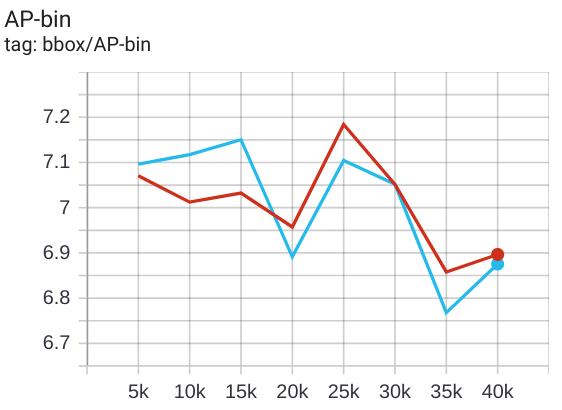
\includegraphics[width=0.6\textwidth]{fig/ap.png}
\vspace{-0.35cm}
\caption{AP on the test dataset during training}
\vspace{-0.4cm}
\label{fig:ap}
\end{figure*}

\begin{figure*}[t]
\centering
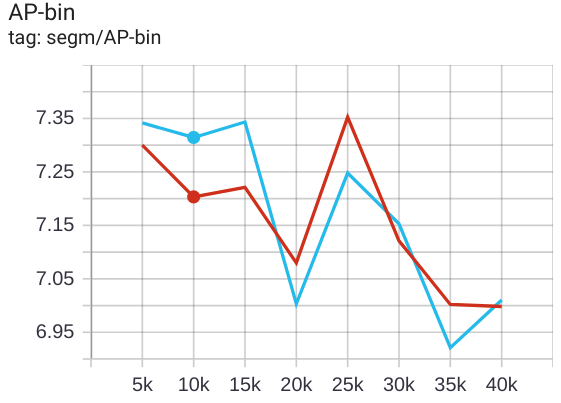
\includegraphics[width=0.6\textwidth]{fig/ap_bin_s.png}
\vspace{-0.35cm}
\caption{AP for object class 'bin' on the test dataset during training}
\vspace{-0.4cm}
\label{fig:ap_bin}
\end{figure*}

\begin{figure*}[t]
\centering
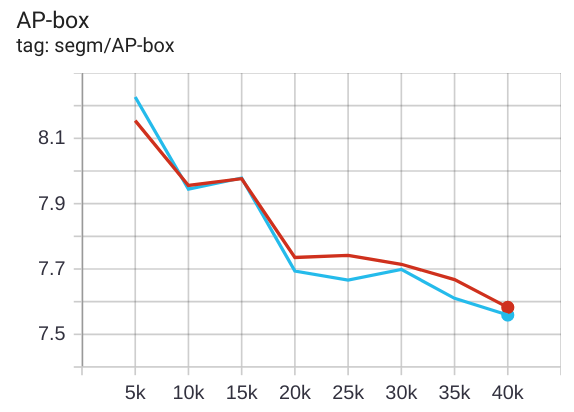
\includegraphics[width=0.6\textwidth]{fig/ap_box_s.png}
\vspace{-0.35cm}
\caption{AP for object class 'box' on the test dataset during training}
\vspace{-0.4cm}
\label{fig:ap_box}
\end{figure*}

\begin{figure*}[t]
\centering
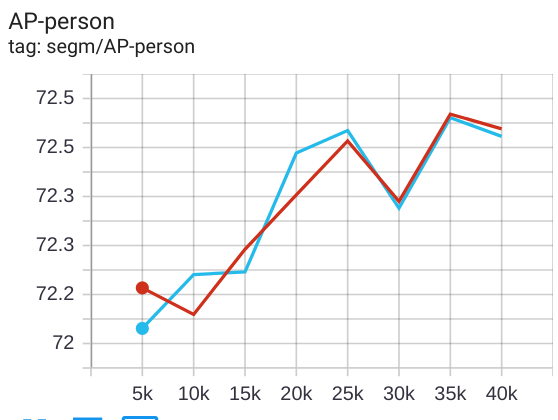
\includegraphics[width=0.6\textwidth]{fig/ap_person_s.png}
\vspace{-0.35cm}
\caption{AP for object class 'person' on the test dataset during training}
\vspace{-0.4cm}
\label{fig:ap_person}
\end{figure*}


 